% Source: graduate-coursework/Daily_Gamecock/Docs/onboarding/Opinion_Editing_Handbook.tex

\documentclass[border=4pt]{standalone}
\usepackage{amssymb}
\usepackage{tikz}
\usepackage{xcolor}
\usetikzlibrary{positioning,shapes.geometric}

\definecolor{garnet}{RGB}{115,0,10}
\definecolor{black}{RGB}{0,0,0}
\definecolor{rose}{RGB}{204,46,64}
\definecolor{atlantic}{RGB}{70,106,159}
\definecolor{congaree}{RGB}{31,65,77}
\definecolor{horseshoe}{RGB}{101,120,11}
\definecolor{neutral90}{RGB}{54,54,54}
\definecolor{neutral70}{RGB}{92,92,92}

\newcommand{\doctitle}{%
    \noindent{\LARGE\bfseries The Daily Gamecock \textit{Opinion}}\\[2pt]
    {\LARGE\bfseries Editing Handbook}\\[4pt]
    {\normalsize J.C. Vaught, Asst. Opinion Editor}\\[-2pt]
    \noindent\rule{\textwidth}{1pt}
    \vspace{8pt}
}

\begin{document}
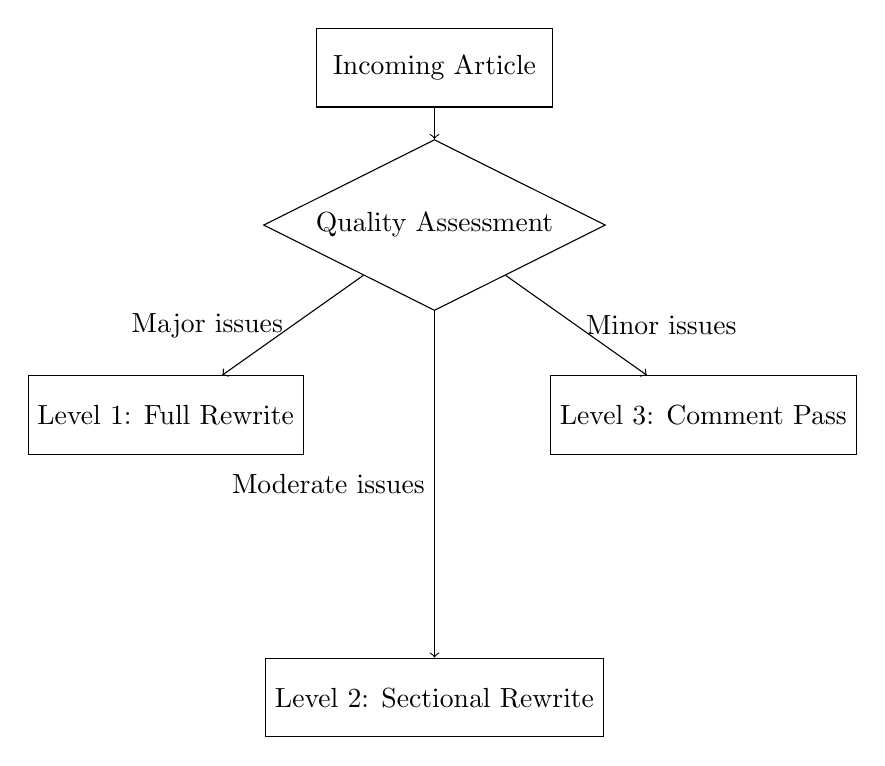
\begin{tikzpicture}[node distance=2cm]
    \node (start) [draw, minimum width=3cm, minimum height=1cm] {Incoming Article};
    \node (assess) [draw, diamond, aspect=2, below of=start, minimum width=3cm, minimum height=2cm] {Quality Assessment};
    \node (level1) [draw, below left of=assess, minimum width=2.5cm, minimum height=1cm, xshift=-2cm, yshift=-1cm] {Level 1: Full Rewrite};
    \node (level2) [draw, below of=assess, minimum width=2.5cm, minimum height=1cm, yshift=-4cm] {Level 2: Sectional Rewrite};
    \node (level3) [draw, below right of=assess, minimum width=2.5cm, minimum height=1cm, xshift=2cm, yshift=-1cm] {Level 3: Comment Pass};

    \draw [->] (start) -- (assess);
    \draw [->] (assess) -- node[anchor=east] {Major issues} (level1);
    \draw [->] (assess) -- node[anchor=east] {Moderate issues} (level2);
    \draw [->] (assess) -- node[anchor=west] {Minor issues} (level3);
\end{tikzpicture}
\end{document}
